\documentclass[tikz,border=6pt]{standalone}
\usepackage{amsmath,amssymb,mathtools,physics,bm,nicefrac,wasysym}
\usepackage{xcolor}

\definecolor{colone}{RGB}{180,60,60}
\definecolor{coltwo}{RGB}{60,110,180}
\definecolor{colthree}{RGB}{60,140,80}

\definecolor{accent}{HTML}{A13D2C}
\definecolor{accent2}{HTML}{2B5F6B}
\definecolor{muted}{HTML}{5A564F}
\definecolor{panel}{HTML}{F8F6F0}
\definecolor{linecol}{HTML}{D8D2C4}
\definecolor{ink}{HTML}{1E1C1A}
\definecolor{astroblue}{HTML}{1B4F72}
\definecolor{astrodark}{HTML}{17202A}
\definecolor{sunyellow}{HTML}{E8A33D}

\usetikzlibrary{calc,arrows.meta,positioning,decorations.pathreplacing,decorations.markings,angles,quotes,shapes.geometric}
\usepackage{tikz-3dplot}

\newcommand{\vecr}{\vec r}
\newcommand{\vecL}{\vec L}
\newcommand{\vecA}{\vec A}
\newcommand{\vecf}{\vec f}
\newcommand{\vecF}{\vec F}
\newcommand{\vecp}{\vec p}
\newcommand{\avg}[1]{\left\langle #1\right\rangle}
\newcommand{\vecx}{\vec x}
\newcommand{\hatn}{\hat n}
\newcommand{\rhat}{\hat r}
\newcommand{\phihat}{\hat\phi}
\newcommand{\thetahat}{\hat\theta}
\newcommand{\note}[1]{\textcolor{blue!60!black}{\textit{[#1]}}}

% Astronomical acronyms
\newcommand{\LST}{\mathrm{LST}}
\newcommand{\GST}{\mathrm{GST}}
\newcommand{\GMST}{\mathrm{GMST}}
\newcommand{\GAST}{\mathrm{GAST}}
\newcommand{\LMST}{\mathrm{LMST}}
\newcommand{\LAST}{\mathrm{LAST}}
\newcommand{\UT}{\mathrm{UT}}
\newcommand{\UTC}{\mathrm{UTC}}
\newcommand{\TAI}{\mathrm{TAI}}
\newcommand{\TT}{\mathrm{TT}}
\newcommand{\TDB}{\mathrm{TDB}}
\newcommand{\JD}{\mathrm{JD}}
\newcommand{\MJD}{\mathrm{MJD}}
\newcommand{\EoT}{\mathrm{EoT}}
\newcommand{\SNR}{\mathrm{SNR}}
\newcommand{\RON}{\mathrm{RON}}

% Helper commands for specific diagrams
\newcommand{\midlinelabel}[3]{
    \node (midlabel) at ($ (#1)!.5!(#2) $) {#3};
    \draw[stealth-] (#1) --  (midlabel);
    \draw[-stealth] (midlabel) -- (#2);
}
\newcommand{\midlinelabell}[3]{
    \node[fill = white, inner sep = 0.2pt, outer sep=3pt] (midlabel) at ($ (#1)!.5!(#2) $) {#3};
    \draw[stealth-] (#1) --  (midlabel);
    \draw[-stealth] (midlabel) -- (#2);
}
\newcommand{\midlinelabelll}[3]{
    \node[fill = white, inner sep = 0.2pt, outer sep=3pt,scale=0.6] (midlabel) at ($ (#1)!.5!(#2) $) {#3};
    \draw[stealth-] (#1) --  (midlabel);
    \draw[-stealth] (midlabel) -- (#2);
}



\begin{document}
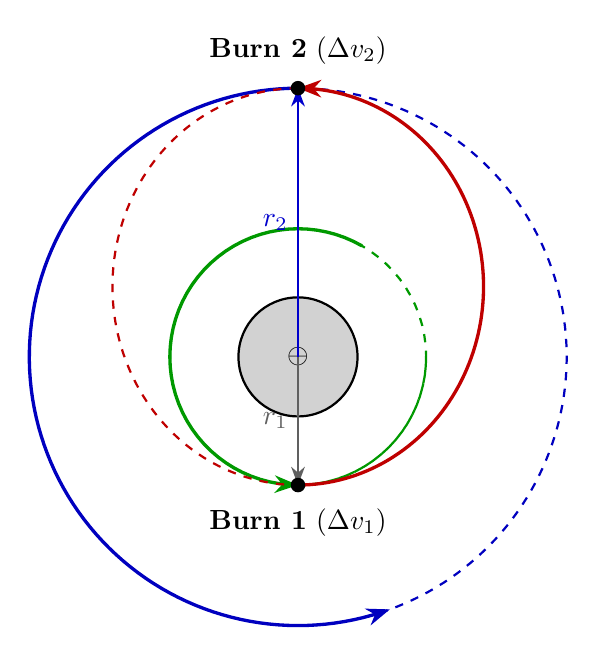
\begin{tikzpicture}[scale=1.05, >=Stealth]
		\def\rone{1.55}
		\def\rtwo{3.25}
		\pgfmathsetmacro{\a}{(\rone+\rtwo)/2}
		\pgfmathsetmacro{\b}{sqrt(\rone*\rtwo)}
		\pgfmathsetmacro{\c}{(\rtwo-\rone)/2}

		% Central body
		\fill[gray!35] (0,0) circle (0.72);
		\draw[thick] (0,0) circle (0.72) node {$\oplus$};

		% Initial orbit
		\draw[green!60!black, dashed, thick, domain=-90:360, samples=100] plot ({\rone*cos(\x)}, {\rone*sin(\x)});
		\draw[green!60!black, very thick, domain=60:270, samples=50, ->] plot ({\rone*cos(\x)}, {\rone*sin(\x)});

		% Final orbit
		\draw[blue!75!black, dashed, thick, domain=-90:90, samples=100] plot ({\rtwo*cos(\x)}, {\rtwo*sin(\x)});
		\draw[blue!75!black, very thick, domain=90:290, samples=100, ->] plot ({\rtwo*cos(\x)}, {\rtwo*sin(\x)});

		% Transfer ellipse
		\draw[red!75!black, dashed, thick, domain=90:270, samples=100] plot ({\b*cos(\x)}, {\c+\a*sin(\x)});
		\draw[red!75!black, very thick, domain=-90:90, samples=100, ->] plot ({\b*cos(\x)}, {\c+\a*sin(\x)});

		% Radial vectors
		\draw[->, gray!75!black, thick] (0,0) -- (0,-\rone) node[midway, left] {$r_1$};
		\draw[->, blue!80!black, thick] (0,0) -- (0,\rtwo) node[midway, left] {$r_2$};

		% Burn points
		\fill (0,-\rone) circle (2.5pt);
		\fill (0,\rtwo) circle (2.5pt);
		\node[below=5pt] at (0,-\rone) {\textbf{Burn 1} ($\Delta v_1$)};
		\node[above=5pt] at (0,\rtwo) {\textbf{Burn 2} ($\Delta v_2$)};
	\end{tikzpicture}
\end{document}
